\section{Merging permutations}
\label{section:Merging permutations}

We are back to merging permutations. 
We show how to transform matching merges to permutation merges.

\begin{proposition}
  \label{proposition:3-merge permutation is NP-complete}
  \textsc{$3$-Merge Permutation} is \NP-complete.
\end{proposition}

\begin{proof}
  We reduce from \textsc{$3$-Merge Matching} (Proposition~\ref{proposition:3-merge matching is NP-complete}).
  Let $\mathcal{M}^{0}$, $\mathcal{M}^{1}$, $\mathcal{M}^{2}$, $\mathcal{M}^{3}$ be four matchings. 
  Write $\mathcal{M}^{i} = (V^i, E^i)$,
  $n_i = |V^i|$ and $m_i = |E^i|$ for $0 \leq i \leq 3$.
  We show how to construct four permutations $\pi^0$, $\pi^1$, $\pi^2$ and $\pi^3$ such that
  the matching $\mathcal{M}^{0}$ is a merge of the matchings $\mathcal{M}^{1}$, $\mathcal{M}^{2}$ and $\mathcal{M}^{3}$
  if and only if
  the permutation $\pi^0$ is a merge of the permutations $\pi^1$, $\pi^2$ and $\pi^3$.

  Define $N_0 = 8m_0 + 1$.
  We first associate a permutation $\pi^0$ to the matching $\mathcal{M}^{0}$.
  Write $V^0 = \{v^0_1, v^0_2, \dots v^0_{n_0}\}$ and
  $E^0 = \{e^0_1, e^0_2, \dots, e^0_{m_0} \}$, where the edges are sorted according to their minimum vertex.
  The permutation $\pi^0$ is defined piecewise and boxes are used to facilitate the reading of the elements.
  Define
  \begin{alignat*}{3}
    &\forall i \in V^0,
    &\quad&
    \pi^0[i] &=&\; \BOXED{i fst}{6N_0 + 2m_0 + 3i} \quad \BOXED{i snd}{6N_0 + 2m_0 + 3i - 2} \\ 
    &\forall e^0_k = (i,j) \in E^0,
    &\quad&
    \pi^0[e^0_k] &=&\; \BOXED{e fst}{2k} \quad \BOXED{e i}{6N_0 + 2m_0 + 3i - 1} \quad \BOXED{e j}{6N_0 + 2m_0 + 3j - 1} \quad \BOXED{e snd}{2k - 1} \\
    \intertext{We have two groups of three separators 
    ($\text{sep}^{k}_{l}$, $1 \leq k \leq 2$ and $1 \leq l \leq 3$) that are defined as follows:}
    &&\quad&
    \pi^0[\text{sep}^{1}_{1}] &=&\; \BOXED{sep 1 1 1}{2N_0 + 2m_0 + 1} \quad \BOXED{sep 1 1 2}{2N_0 + 2m_0 + 2} \quad \dots \quad \BOXED{sep 1 1 N0}{2N_0 + 2m_0 + N_0} \\ 
    &&\quad&
    \pi^0[\text{sep}^{1}_{2}] &=&\; \BOXED{sep 1 2 1}{N_0 + 2m_0 + 1} \quad \BOXED{sep 1 2 2}{N_0 + 2m_0 + 2} \quad \dots \quad \BOXED{sep 1 2 N0}{N_0 + 2m_0 + N_0} \\ 
    &&\quad&
    \pi^0[\text{sep}^{1}_{3}] &=&\; \BOXED{sep 1 3 1}{2m_0 + 1} \quad \BOXED{sep 1 3 2}{2m_0 + 2} \quad \dots \quad \BOXED{sep 1 3 N0}{2m_0 + N_0} \\ 
    &&\quad&
    \pi^0[\text{sep}^{2}_{1}] &=&\; \BOXED{sep 2 1 1}{5N_0 + 2m_0 + 1} \quad \BOXED{sep 2 1 2}{5N_0 + 2m_0 + 2} \quad \dots \quad \BOXED{sep 2 1 N0}{5N_0 + 2m_0 + N_0} \\ 
    &&\quad&
    \pi^0[\text{sep}^{2}_{2}] &=&\; \BOXED{sep 2 2 1}{4N_0 + 2m_0 + 1} \quad \BOXED{sep 2 2 2}{4N_0 + 2m_0 + 2} \quad \dots \quad \BOXED{sep 2 2 N0}{4N_0 + 2m_0 + N_0} \\ 
    &&\quad&
    \pi^0[\text{sep}^{2}_{3}] &=&\; \BOXED{sep 2 3 1}{3N_0 + 2m_0 + 1} \quad \BOXED{sep 2 3 2}{3N_0 + 2m_0 + 2} \quad \dots \quad \BOXED{sep 2 3 N0}{3N_0 + 2m_0 + N_0}\text{.}
    \intertext{Define}
    &&\quad&
    \pi^0[V^0] &=&\; \pi^0[1] \;\; \pi^0[2] \;\; \dots \;\; \pi^0[2m_0] \\
    &&\quad&
    \pi^0[E^0] &=&\; \pi^0[e^0_1] \;\; \pi^0[e^0_2] \; \dots \;\; \pi^0[e^0_{m_0}] \\
    &&\quad&
    \pi^0[\text{sep}^{1}] &=&\; \pi^0[\text{sep}^{1}_{1}] \;\; \pi^0[\text{sep}^{1}_{2}] \;\; \pi^0[\text{sep}^{1}_{3}] \\
    &&\quad&
    \pi^0[\text{sep}^{2}] &=&\; \pi^0[\text{sep}^{2}_{1}] \;\; \pi^0[\text{sep}^{2}_{2}] \;\; \pi^0[\text{sep}^{2}_{3}]\text{.}
  \end{alignat*}
  In other words,
  $\pi^0[V^0]$ is the direct sum of $2m_0$ decreasing permutations
  that are all order-isomorphic to $21$,
  $\pi^0[E^0]$ is the direct sum of $m_0$ permutations that are all
  order-isomorphic to $2341$, and
  both $\pi^0[\text{sep}^{1}]$ and $\pi^0[\text{sep}^{2}]$ are the skew sums
  of $3$ permutations that are all order-isomorphic to $12 \dots N_0$.
  The permutations $\pi^0$ is defined as follows:
  $$
  \pi^0 = \pi^0[V^0] \;\; \pi^0[\text{sep}^{1}] \;\; \pi^0[E^0] \;\; \pi^0[\text{sep}^{2}]\text{.}
  $$
  See Fig.\ref{fig:example-merge-permutation-pi0} for an example.

  \begin{figure}
  \centering
  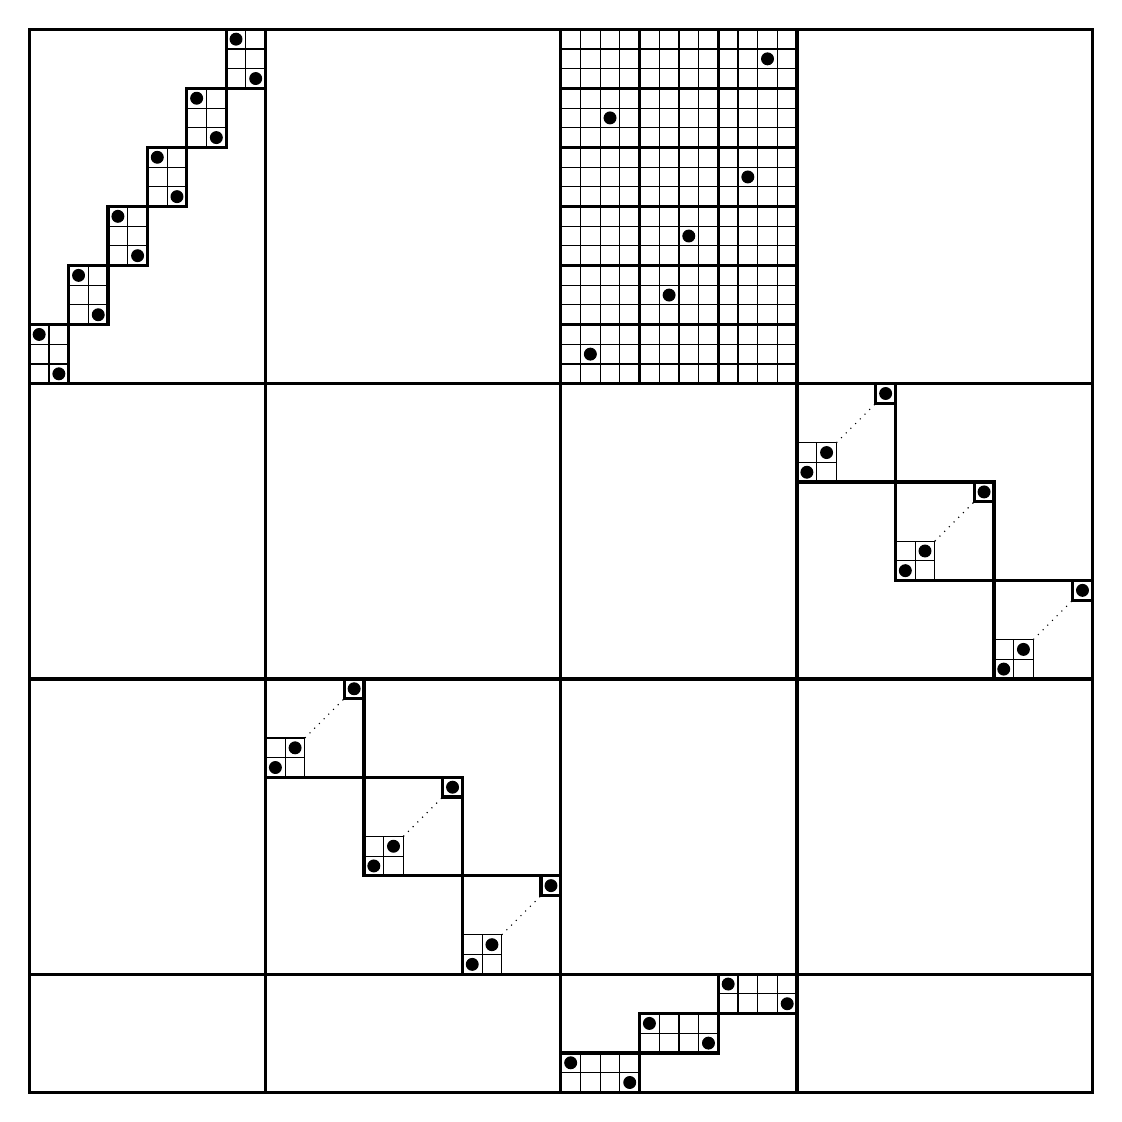
\begin{tikzpicture}
  [
    scale=.25,
  ]
  
  % grid
  \draw [step=1.0, black, very thick] (0,0) rectangle (54,54);
  \draw [step=1.0, black, very thick] (12,0) -- (12,54);
  \draw [step=1.0, black, very thick] (27,0) -- (27,54);
  \draw [step=1.0, black, very thick] (39,0) -- (39,54);
  \draw [step=1.0, black, very thick] (0,6) -- (54,6);
  \draw [step=1.0, black, very thick] (0,21) -- (54,21);
  \draw [step=1.0, black, very thick] (0,36) -- (54,36);

  % vertices
  \def\y{36}
  \foreach \i in {1,2,...,6} {
    \draw [step=1.0, black] (2*\i - 2, \y + 3*\i - 3) grid (2*\i, \y + 3*\i);
    \draw [black, very thick] (2*\i - 2, \y + 3*\i - 3) rectangle (2*\i, \y + 3*\i);
    \draw [fill=black] (2*\i - 1.5, \y + 3*\i - .5) circle (0.3);
    \draw [fill=black] (2*\i - .5, \y - 2 + 3*\i - .5) circle (0.3);
  }
  
  % edges
  \draw [step=1.0, black] (27,36) grid (39, 54);
  \draw [black, very thick] (27,36) rectangle (39, 54);
  \foreach \k/\i/\j in {1/1/5,2/2/3,3/4/6} {
    \draw [step=1.0, black] (4*\k + 23, 2*\k - 2) grid (4*\k + 27, 2*\k);
    \draw [black, very thick] (4*\k + 23, 2*\k - 2) rectangle (4*\k + 27, 2*\k);
    \draw [fill=black] (4*\k + 23 + 1 - .5, 2*\k - .5) circle (0.3);
    \draw [fill=black] (4*\k + 23 + 4 - .5, 2*\k - 1 - .5) circle (0.3);
    \draw [fill=black] (4*\k + 23 + 2 - .5, 36 + 3*\i - 1 - .5) circle (0.3);
    \draw [fill=black] (4*\k + 23 + 3 - .5, 36 + 3*\j - 1 - .5) circle (0.3);
  }
  % horizontal
  \draw [black, very thick] (31, 36) -- (31, 54);
  \draw [black, very thick] (35, 36) -- (35, 54);
  % vertical
  \draw [black, very thick] (27, 39) -- (39, 39);
  \draw [black, very thick] (27, 42) -- (39, 42);
  \draw [black, very thick] (27, 45) -- (39, 45);
  \draw [black, very thick] (27, 48) -- (39, 48);
  \draw [black, very thick] (27, 51) -- (39, 51);


  % separators 2
  \def\x{39}
  \def\y{31}
  \foreach \i in {1,2,3} {
    \def\xs2{\x + 5*\i - 5}
    \def\ys2{\y - 5*\i + 5}
    \draw [black, very thick] (\xs2, \ys2) rectangle (\xs2 + 5, \ys2 + 5);
    \draw [step=1.0, black] (\xs2, \ys2) grid (\xs2 + 2, \ys2 + 2);
    \draw [dotted] (\xs2 + 2, \ys2 + 2) -- (\xs2 + 4, \ys2 + 4);
    \draw [black, very thick] (\xs2 + 4, \ys2 + 4) rectangle (\xs2 + 5, \ys2 + 5);
    \draw [fill=black] (\xs2 + .5, \ys2 + .5) circle (0.3);
    \draw [fill=black] (\xs2 + 1.5, \ys2 + 1.5) circle (0.3);
    \draw [fill=black] (\xs2 + 4.5, \ys2 + 4.5) circle (0.3);
  }

  % separators 1
  \def\x{12}
  \def\y{16}
  \foreach \i in {1,2,3} {
    \def\xs2{\x + 5*\i - 5}
    \def\ys2{\y - 5*\i + 5}
    \draw [black, very thick] (\xs2, \ys2) rectangle (\xs2 + 5, \ys2 + 5);
    \draw [step=1.0, black] (\xs2, \ys2) grid (\xs2 + 2, \ys2 + 2);
    \draw [dotted] (\xs2 + 2, \ys2 + 2) -- (\xs2 + 4, \ys2 + 4);
    \draw [black, very thick] (\xs2 + 4, \ys2 + 4) rectangle (\xs2 + 5, \ys2 + 5);
    \draw [fill=black] (\xs2 + .5, \ys2 + .5) circle (0.3);
    \draw [fill=black] (\xs2 + 1.5, \ys2 + 1.5) circle (0.3);
    \draw [fill=black] (\xs2 + 4.5, \ys2 + 4.5) circle (0.3);
  }

  \end{tikzpicture}
\end{figure}

  We now turn to associating a permutation $\pi^l$
  to the matching $\mathcal{M}^l = (V^l, E^l)$, $1 \leq l \leq 3$.
  The construction, as a whole, follows the same line as of $\pi^0$,
  the main difference being the \emph{separators}
  $\pi^l[\text{sep}^{1}]$ and
  $\pi^l[\text{sep}^{1}]$ that are both simplified.
  Write $V^k = \{v^l_1, v^l_2, \dots v^l_{n_0}\}$ and
  $E^0 = \{e^l_1, e^l_2, \dots, e^l_{m_l} \}$, where the edges are sorted according to their minimum vertex.
  Define
  \begin{alignat*}{3}
    &\forall i \in V^l,
    &\quad&
    \pi^l[i] &=&\; \BOXED{l i fst}{2N_0 + 2m_l + 3i} \quad \BOXED{l i snd}{2N_0 + 2m_l + 3i - 2} \\ 
    &\forall e^0_k = (i,j) \in E^l,
    &\quad&
    \pi^l[e^l_k] &=&\; \BOXED{l e fst}{2k} \quad \BOXED{l e i}{2N_0 + 2m_l + 3i - 1} \quad \BOXED{l e j}{2N_0 + 2m_l + 3j - 1} \quad \BOXED{l e snd}{2k - 1} \\
    \intertext{We have two groups of three separators 
    ($\text{sep}^{k}_{l}$, $1 \leq k \leq 2$ and $1 \leq l \leq 3$) that are defined as follows:}
    &&\quad&
    \pi^l[\text{sep}^{1}] &=&\; \BOXED{l sep 1 1}{2m_0 + 1} \quad \BOXED{l sep 1 2}{2m_0 + 2} \quad \dots \quad \BOXED{l sep 1 N0}{2m_0 + N_0} \\ 
    &&\quad&
    \pi^l[\text{sep}^{2}] &=&\; \BOXED{l sep 2 1}{N_0 + 2m_0 + 1} \quad \BOXED{l sep 2 2}{N_0 + 2m_0 + 2} \quad \dots \quad \BOXED{l sep 2 N0}{N_0 + 2m_0 + N_0}\text{.} \\ 
    \intertext{Define}
    &&\quad&
    \pi^l[V^0] &=&\; \pi^0[1] \;\; \pi^0[2] \;\; \dots \;\; \pi^0[2m_0] \\
    &&\quad&
    \pi^l[E^0] &=&\; \pi^0[e^0_1] \;\; \pi^0[e^0_2] \; \dots \;\; \pi^0[e^0_{m_0}]\text{.}
  \end{alignat*}
  In other words,
  $\pi^l[V^l]$ is the direct sum of $2m_l$ decreasing permutations
  that are all order-isomorphic to $21$,
  $\pi^l[E^l]$ is the direct sum of $m_l$ permutations that are all
  order-isomorphic to $2341$, and
  both $\pi^l[\text{sep}^{1}]$ and $\pi^l[\text{sep}^{2}]$ are order-isomorphic to $12 \dots N_0$.
  See Fig.\ref{fig:example-merge-permutation-pi1} for an example.
  The permutations $\pi^l$ is defined as follows:
  $$
  \pi^l = \pi^l[V^l] \;\; \pi^l[\text{sep}^{1}] \;\; \pi^l[E^l] \;\; \pi^l[\text{sep}^{2}]\text{.}
  $$

  \begin{figure}
  \centering
  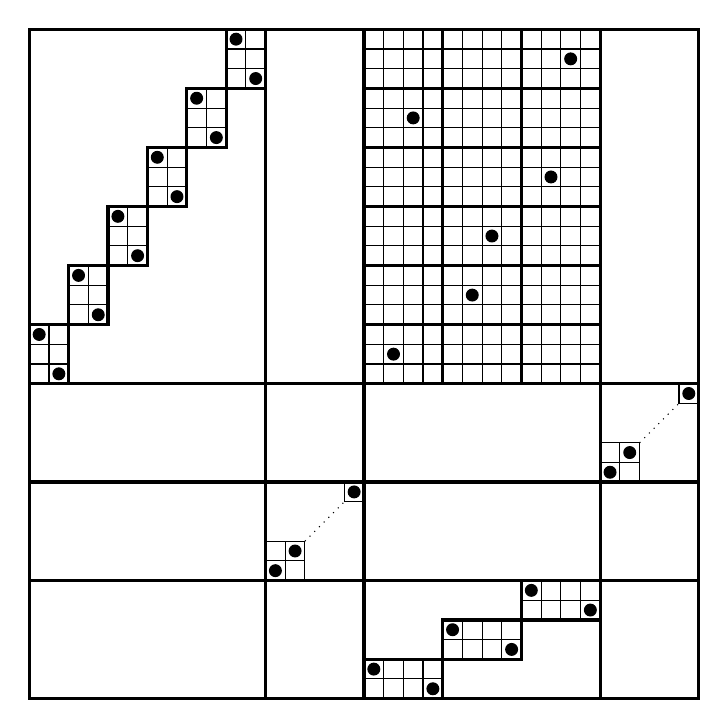
\begin{tikzpicture}
  [
    scale=.25,
  ]
    
    % grid
    \draw [step=1.0, black, very thick] (0,0) rectangle (34,34);
    \draw [step=1.0, black, very thick] (12,0) -- (12,34);
    \draw [step=1.0, black, very thick] (17,0) -- (17,34);
    \draw [step=1.0, black, very thick] (29,0) -- (29,34);
    \draw [step=1.0, black, very thick] (0,6) -- (34,6);
    \draw [step=1.0, black, very thick] (0,16) -- (34,16);
    \draw [step=1.0, black, very thick] (0,11) -- (34,11);

    % vertices
    \def\y{16}
    \foreach \i in {1,2,...,6} {
      \draw [step=1.0, black] (2*\i - 2, \y + 3*\i - 3) grid (2*\i, \y + 3*\i);
      \draw [black, very thick] (2*\i - 2, \y + 3*\i - 3) rectangle (2*\i, \y + 3*\i);
      \draw [fill=black] (2*\i - 1.5, \y + 3*\i - .5) circle (0.3);
      \draw [fill=black] (2*\i - .5, \y - 2 + 3*\i - .5) circle (0.3);
    }
    
    % edges
    \draw [step=1.0, black] (17,16) grid (29, 34);
    \draw [black, very thick] (17,16) rectangle (29, 34);
    \foreach \k/\i/\j in {1/1/5,2/2/3,3/4/6} {
      \draw [step=1.0, black] (4*\k + 13, 2*\k - 2) grid (4*\k + 17, 2*\k);
      \draw [black, very thick] (4*\k + 13, 2*\k - 2) rectangle (4*\k + 17, 2*\k);
      \draw [fill=black] (4*\k + 13 + 1 - .5, 2*\k - .5) circle (0.3);
      \draw [fill=black] (4*\k + 13 + 4 - .5, 2*\k - 1 - .5) circle (0.3);
      \draw [fill=black] (4*\k + 13 + 2 - .5, 16 + 3*\i - 1 - .5) circle (0.3);
      \draw [fill=black] (4*\k + 13 + 3 - .5, 16 + 3*\j - 1 - .5) circle (0.3);
    }
    % vertical
    \draw [black, very thick] (21, 16) -- (21, 34);
    \draw [black, very thick] (25, 16) -- (25, 34);
    % horizontal
    \draw [black, very thick] (17, 19) -- (29, 19);
    \draw [black, very thick] (17, 22) -- (29, 22);
    \draw [black, very thick] (17, 25) -- (29, 25);
    \draw [black, very thick] (17, 28) -- (29, 28); 
    \draw [black, very thick] (17, 31) -- (29, 31);

    % separators 2
    \def\x{29}
    \def\y{11}
    \def\i{1}
    \def\xs2{\x + 5*\i - 5}
    \def\ys2{\y - 5*\i + 5}
    \draw [black, very thick] (\xs2, \ys2) rectangle (\xs2 + 5, \ys2 + 5);
    \draw [step=1.0, black] (\xs2, \ys2) grid (\xs2 + 2, \ys2 + 2);
    \draw [dotted] (\xs2 + 2, \ys2 + 2) -- (\xs2 + 4, \ys2 + 4);
    \draw [black] (\xs2 + 4, \ys2 + 4) rectangle (\xs2 + 5, \ys2 + 5);
    \draw [fill=black] (\xs2 + .5, \ys2 + .5) circle (0.3);
    \draw [fill=black] (\xs2 + 1.5, \ys2 + 1.5) circle (0.3);
    \draw [fill=black] (\xs2 + 4.5, \ys2 + 4.5) circle (0.3);

    % separators 1
    \def\x{12}
    \def\y{6}
    \def\i{1}
    \def\xs2{\x + 5*\i - 5}
    \def\ys2{\y - 5*\i + 5}
    \draw [black, very thick] (\xs2, \ys2) rectangle (\xs2 + 5, \ys2 + 5);
    \draw [step=1.0, black] (\xs2, \ys2) grid (\xs2 + 2, \ys2 + 2);
    \draw [dotted] (\xs2 + 2, \ys2 + 2) -- (\xs2 + 4, \ys2 + 4);
    \draw [black] (\xs2 + 4, \ys2 + 4) rectangle (\xs2 + 5, \ys2 + 5);
    \draw [fill=black] (\xs2 + .5, \ys2 + .5) circle (0.3);
    \draw [fill=black] (\xs2 + 1.5, \ys2 + 1.5) circle (0.3);
    \draw [fill=black] (\xs2 + 4.5, \ys2 + 4.5) circle (0.3);
  \end{tikzpicture}

  \caption{\label{fig:example-merge-permutation-pi1}
  Transforming the matching \raisebox{-.25cm}{\EXAMPLEM} into the permutation $\pi^i$, $i \neq 0$..
}% end caption
\end{figure}

  Clearly our construction can be carried on in polynomial time.
  Indeed, we have
  $|\pi^0| = 6N_0 + 8m_0 = 56m_0 + 1$
  and
  $|\pi^l| = 2N_0 + 8m_l = 16m_0 + 8m_l$,
  $1 \leq l \leq 3$.
  We claim that the matching $\mathcal{M}^0$ is a merge of the matchings
  $\mathcal{M}^1$, $\mathcal{M}^2$ and $\mathcal{M}^3$
  if and only if the permutation
  $\pi^0$ is a merge of the permutations $\pi^1$, $\pi^2$ and $\pi^3$.

  Suppose first 
  that the matching $\mathcal{M}^0$ is a merge of the matchings
  $\mathcal{M}^1$, $\mathcal{M}^2$ and $\mathcal{M}^3$.
  Therefore, there exists a $3$-coloring $c : V^0 \to [3]$
  and functions $f_l : V^l \to V^0$ such that, for every $1 \leq l \leq 3$,
  (i) $i < j$ implies $f_l(i) < f_l(j)$ and  
  (ii) $(i, j) \in E^l$ implies $(f(i), f(j)) \in E^0$ and $(c \circ f)(i) = (c \circ f)(j) = l$.
  Let us now define a $3$-colouring of $\pi^0$ as follows.
  \begin{itemize}
    \item \textbf{Sequences $\pi^0[1], \pi^0[2], \dots, \pi^0[2m_0]$}.
    For every $1 \leq i \leq 2m_0$, color the two integers of $\pi^0[i]$ with color $c(i)$.
    \item \textbf{Sequences $\pi^0[\text{sep}^{1}_{l}]$, $1 \leq l \leq 3$}.
    Color the integers of $\pi^0[\text{sep}^{1}_{l}]$ with colour $l$.
    \item \textbf{Sequences $\pi^0[e^0_1], \pi^0[e^0_2], \dots, \pi^0[e^0_{m_0}]$}.
    For every $1 \leq k \leq m_0$, color the four integers of $\pi^0[e^0_k = (i, j)]$ with color $c(i) = c(j)$.
    \item \textbf{Sequences $\pi^0[\text{sep}^{2}_{l}]$, $1 \leq l \leq 3$}.
    Color the integers of $\pi^0[\text{sep}^{2}_{l}]$ with colour $l$.
  \end{itemize}
  The reader is invited to check that, for every $1 \leq l \leq 3$,
  the $l$-coloured pattern of $\pi^0$ is order-isomorphic to $\pi^l$.

  Conversely, suppose that 
  $\pi^0$ is a merge of the permutations $\pi^1$, $\pi^2$ and $\pi^3$.
  Therefore, there exists a $3$-coloring $c': [56m_0 + 1] \to [3]$
  such that, for every $1 \leq l \leq 3$,
  the $l$-coloured pattern of $\pi^0$ is order-isomorphic to $\pi^l$.
  Let us focus on $\pi^l$ for some $1 \leq i \leq k$.
  Recall that
  $\pi^l = \pi^l[V^l] \;\; \pi^l[\text{sep}^{1}] \;\; \pi^l[E^l] \;\; \pi^l[\text{sep}^{2}]$
  where both
  $\pi^l[\text{sep}^{1}]$ and $\pi^l[\text{sep}^{2}]$
  are increasing sequence of length $N_0$.
  We now oberve that
  $\pi^l[\text{sep}^{1}] \;\; \pi^l[\text{sep}^{2}]$ is an increasing sequence of length $2N_0$.
  Combining this observation with  
  $N_0 > |\pi^0[V^0]| + |\pi^0[E^0]|$,
  we obtain that the 
  (i)  and that each increasing sequence of $\pi^0[\text{sep}^{1}]$
  (\emph{i.e.}, $\pi^0[\text{sep}^{1}_{1}]$, $\pi^0[\text{sep}^{1}_{2}]$ and $\pi^0[\text{sep}^{1}_{3}]$)
  is coloured with a distinct color, and that
  (ii) each increasing sequence of $\pi^0[\text{sep}^{2}]$
  (\emph{i.e.}, $\pi^0[\text{sep}^{2}_{1}]$, $\pi^0[\text{sep}^{2}_{2}]$ and $\pi^0[\text{sep}^{2}_{3}]$)
  is coloured with a distinct color.
  Then it folows that 
  $2m_l$ sequences of $\pi^0[V^0] = \pi^0[1] \;\; \pi^0[2] \;\; \dots \;\; \pi^0[2m_0]$ are colored with color $l$ 
  and that 
  $m_l$ sequences of $\pi^0[E^0] = \pi^0[e^0_1] \;\; \pi^0[e^0_2] \; \dots \;\; \pi^0[e^0_{m_0}]$
  are colored with color $l$.
  Therefore, 
  we conclude that the matching $\mathcal{M}^0$ is a merge 
  of the matchings $\mathcal{M}^1$, $\mathcal{M}^2$ and $\mathcal{M}^3$.
  \qed
\end{proof}

It is worth noticing that, according to the proof
Proposition~\ref{proposition:3-merge permutation is NP-complete},
any improvement on Proposition~\ref{proposition:3-merge matching is NP-complete}
would immediately propagate to \textsc{$k$-permutation coloring}.
